%!TEX root = ../main.tex

\chapter{Seeding the Epilepsy Network from iEEG to Resting State fMRI}
\label{chapter-seeding-iEEG-to-fmri}
In this chapter, we investigate the concordance between infra-slow activities at the locations of iEEG recordings and the infra-slow resting-state fMRI brain connectivity using quantitative analysis based on Granger causality and graph theory. Results show the correlation between the two at the corresponding locations around the seizure onset. 

\section{Introduction}
Intracranial EEG (iEEG) is the predominant invasive method for surgical resection decision making \citep{shah2014invasive}. Resting state fMRI (rsfMRI) is a non-invasive method that records the blood oxygen level dependent (BOLD) signals, and is increasingly applied to study brain activities and characterize network dysfunctions \citep{centeno2014network}. The main objective of iEEG, and any other neuroimaging modalities is to localize the seizure focus for resection.

Simultaneous scalp EEG-fMRI has shown some promising results in localizing seizure source \citep{bettus2011interictal, bagshaw2006correspondence,su2019fmri,an2013electroencephalography,thornton2010eeg}. The scalp EEG records activity of pyramidal neurons near the surface of the brain and is relatively insensitive to deep brain structures. Due to lower spatial resolution compared to iEEG, scalp EEG may not record epileptiform activities originating from smaller regions. Aghakhani et. al studied the potential of simultaneous iEEG-fMRI for seizure onset localization  \citep{aghakhani2015co}. This approach may not record exact BOLD signals because of signal distortion near the implanted electrodes. Some studies have discussed coupling of iEEG classical frequencies ($\alpha$, $\beta$, $\theta$ and $\gamma$) with spontaneous fMRI BOLD signals \citep{bettus2011interictal, shah2019characterizing}. Recently, one of our group participated in a study that directly correlated infraslow scalp EEG with spontaneous fMRI BOLD signals as well \citep{grooms2017infraslow}. The signal was subtle and required averaging the rsfMRI across a group of normal subjects.

%Independent component analysis (ICA) method have been used in some studies to localize the source using fMRI \citep{hunyadi2013ica, gil2020beyond, ebrahimzadeh2019component, zhang2020establishing}. ICA represents the source in blobs and does not show the connectivity between different brain networks. 

%Several studies have demonstrated the links between neuronal activity recorded by iEEG and BOLD signal modulations \citep{ aghakhani2015co, su2019fmri}. Computational studies have demonstrated an optimal coherence of gamma oscillations with $< 0.1 $ Hz fluctuations \citep{wang2012electrophysiological}. 

%Study by Shah et. al has shown direct concurrent spontaneous fluctuations of neuronal activity and BOLD signal in monkey’s visual cortex using simultaneous fMRI and intracortical electrophysiological recording at rest \citep{shah2019characterizing}.

By seeding the ictal iEEG network into resting state fMRI, this study presents correlation between infraslow iEEG at the locations of the seizure onset (SO) electrodes to the corresponding voxels of rsfMRI, and the functional connection of fMRI siezure voxel to the whole brain using functional connectivity methodologies, including Granger causality and graph theoretical measures. 

%We also study the functional connection of fMRI seizure voxel to whole brain.

%Limited studies in the literature have either shown correspondence with classical frequency \citep{bettus2011interictal}, or identify blobs rather than networks, and have not been directly correlated with epilepsy networks in fine detail as EEG.


\section{Materials and methods}
\label{sec:methods}

\subsection{Patient information}
The study is based on the preictal and interictal iEEG recordings and fMRI scans from patient A discussed in the previous chapter. The patient lacked any obvious anatomical lesion on 3 Tesla MRI but clinical confidence in the site of seizure onset was assessed by contemporary iEEG, and positron emission tomography (PET). The patient has been in complete remission for 6 years following laser ablation along the track of the electrode that recorded electrographic seizure onset.

\subsection{Data acquisition}
iEEG were recorded from implantation of a total 128 depth electrodes, subdural grids, or strip electrodes using the Natus XLTEK system in various hypothesized temporal, frontal and motor cortices. The iEEG recordings with final sampling rate of 500 Hz were downloaded in wideband EDF (European data format) data format for further analysis.

Both T1 structural scan and resting state fMRI (T2*) were obtained at the Emory University Neuroimaging facility using a 3T SIEMENs scanner a few months before and after the implantation of depth electrodes. The head was scanned using scanning sequence ‘EP’, slice thickness of 2mm, repetition time 720ms, Echo Time 32ms and Flip Angle 52. T1 or the anatomical scan was done using the scanning sequence GRIR with slice thickness 0.8000mm, Repetition Time 2300ms, Echo Time 2.7500ms and flip angle 8, then repeated following the implant.

\subsection{Data pre-processing}
IEEG data were preprocessed in EEGLAB \citep{delorme2004eeglab}. Bad channels were removed and the data were low pass filtered in the range of 0.01 Hz to 10 Hz using default FIR filter. The data were not downsampled. Further causal relationship and network analysis was carried out on temporal mean removed iEEG data.

Preprocessing of fMRI data was carried out in SPM12 and MATLAB based Conn-functional connectivity toolbox. Dicom files were imported to Nifti in SPM12 \citep{ashburner2014spm12} and further analyses were carried out in Conn-functional connectivity Toolbox \citep{whitfield2012conn}. Functional realignment and unwarp was done at first for subject motion estimation and correction. Functional center to (0,0,0) co-ordinates (translation), functional slice timing correction, functional outlier detection (ART-based identification of outlier scans for scrubbing), functional direct segmentation and normalization (simultaneous Gray/white/CSF segmentation and MNI normalization) were done as the part of the preprocessing. For structural data, translation and structural segmentation and normalization (simultaneous Gray/white/CSF segmentation and normalization) were carried out. TRs with a motion threshold greater than 0.9mm were discarded.

BOLD signal change time series was extracted from the exact locations as those of iEEG electrode contacts. T1 images of the patient before electrode implantation and after electrode implantation were co-registered using SPM clinical toolbox \citep{rorden2012age}. 3D electrode contacts were identified in CT scan by neurophysiologist and MRI physicist. Those electrode contacts were manually recognized on normalized T1 by overlaying normalized T1 obtained after the electrode implantation. MNI coordinates for electrode contacts were obtained based on AAL atlas in MRICRON  \citep{rorden2000stereotaxic}. ROI time-series were extracted, for different radius spherical masks, from these coordinates as center, in the MARSBAR toolbox in SPM \citep{eickhoff2005new}. The normalized, segmented gray matter from the T1 scan of the same patient was used as a mask to extract voxelwise BOLD signal change time-series, for whole brain analysis. The surface file generated from the T1 of the same patient is used for displaying the voxelwise causality relationship in BrainNet viewer \citep{xia2013brainnet}.

\subsection{Granger causality and graph measures}
We computed Granger causality and graph measures to examine time-varying infra-slow causal interactions among multi-channel digitized iEEG time series and BOLD signal time series \citep{dhamala2008analyzing}. The parametric pairwise Granger causality was computed using MVAR modelling in frequency domain in the infa-slow frequency range 0.01-0.2 Hz for iEEG and in range of 0.08-0.8 Hz for spontaneous BOLD signal time-series. The optimal model order for each calculation was obtained by comparing the power between parametric and non-parametric methods \citep{adhikari2013localizing}. The time domain Granger causality measures was obtained by integrating in the infa-slow frequency range \citep{geweke1982measurement}.

Graph measures were computed from the time domain Granger Causality matrix as the adjacency matrix using BCT toolbox \citep{rubinov2010complex} with threshold of 40\% above the maximum granger causal flow. Electrodes are considered as the node and the causal relations between nodes are considered as the edges. Three centrality measures, betweenness, degree and closeness were computed to study the importance of SO electrodes in the network. Clustering coefficient was computed as the measure of segregation of the network.

The statistical significance of the Granger causality measures and graph measures were done by resampling techniques built on a baseline null hypothesis distribution. The threshold value of each of the measures were computed from surrogate data methods by using data permutation calculating GC values and a gamma function fit to a distribution of maximum GC values for each permutation. This threshold was designed to reject a null hypothesis of no interdependence at a significance level of $p<10^-6$ \citep{adhikari2013localizing}.


\section{Results}
\label{sec:results}

\subsection{Granger causality}
To compare the causal relationship in identical frequency range for both the iEEG and spontaneous BOLD signal, we computed Granger causal measures. Figure \ref{fig:GC_EEG} shows the source, sink and total GC from temporal mean removed iEEG time-series. These measures were computed in the infra-slow frequency range of 0.01 to 0.2 Hz from interictal iEEG recordings.  The electrodes highlighted with a red box are SO electrodes, RSMAcd3 and RSMAcd4. These electrodes have maximum sink (causal inflow) and total GC (total causal flow) out of the 119 implanted electrodes. Only 35 representative electrodes are shown in the figure.

For similar analysis of the fMRI, we use corresponding electrode locations manually based on identified images on CT (computed tomography). The MNI co-ordinates of these locations are presented in Table \ref{table:channel_mni_coordinates_map} in the appendix section. Average BOLD signal change were extracted at the 4mm radius sphere around these MNI coordinates. There was no overlap of areas between two consecutive regions of interest (ROI). Causal relations were computed between BOLD signal change time-series from these areas and integrated in the frequency range 0.08-0.8 Hz. Figure \ref{fig:GC_BOLD} show that the total GC and sink activities are visibly clustered around the SO electrodes, and one of the SO electrode are ranked topmost in terms of total causal flow out of the 35 selected regions.

\begin{figure*}
\centerline{
	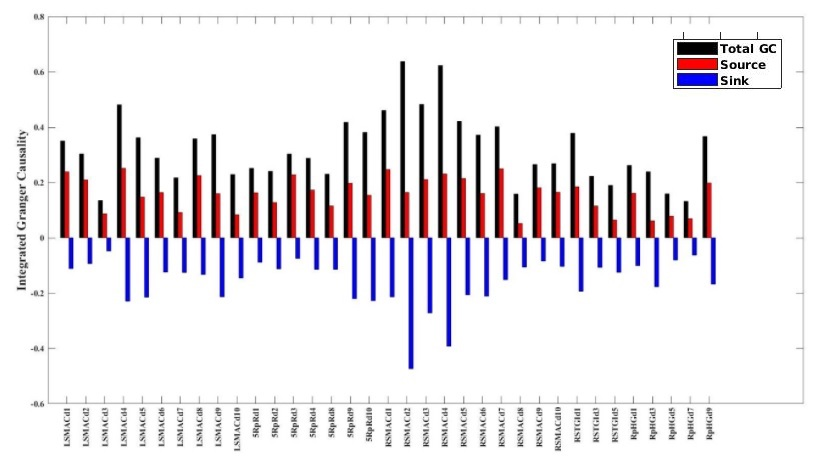
\includegraphics[height =3.5in]{Plots/GC_iEEG.jpg}
	}
	\caption{The total GC, source, sink activity as calculated from iEEG time series. RSMAcd3 and RSMAcd4 are two electrode contacts identified as EZ focus by neurologists. These two contacts are ranked among the highest for GC total and sink activity
	\label{fig:GC_EEG}
}
\end{figure*}

\begin{figure*}
\centerline{
	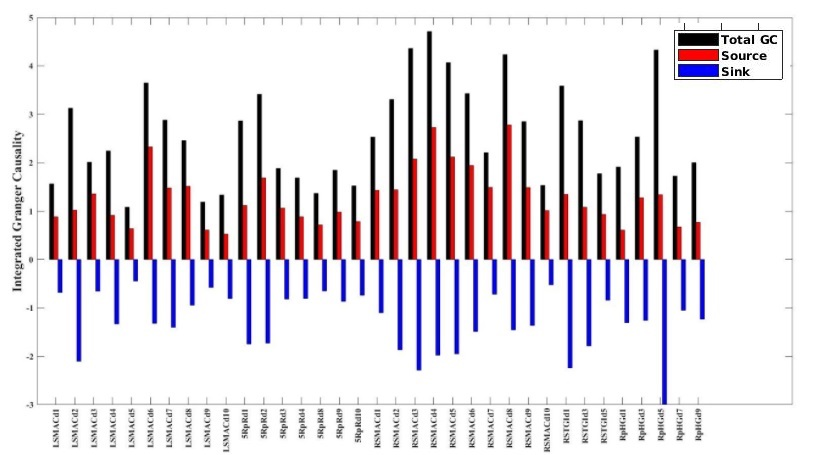
\includegraphics[height =3.5in]{Plots/GC_BOLD.jpg}
	}
	\caption{ Total Granger causality, source, sink activity as obtained from BOLD time series. RSMAcd3 and RSMAcd4 have comparatively higher Total GC and sink activity
	\label{fig:GC_BOLD}
}
\end{figure*}


\subsection{Graph theory}
Figure \ref{fig:betweenness_fmri_eeg}[a-b] shows the betweenness measure computed for iEEG and fMRI networks. The SO electrodes and the corresponding voxels RSMAcd is ranked top among 35 selected electrodes. The edges in the figure represents the strongest connection which was observed between RSMAcd and LSMAcd electrodes, located in opposite hemisphere. The next stronger connection of SO is with the hippocampus in both the networks, which is also considered as the generator of temporal epilespy \citep{avoli2007epileptic}. The connection is stronger in fMRI network compared to the iEEG network.


\begin{figure}%
    \centering
    a) {{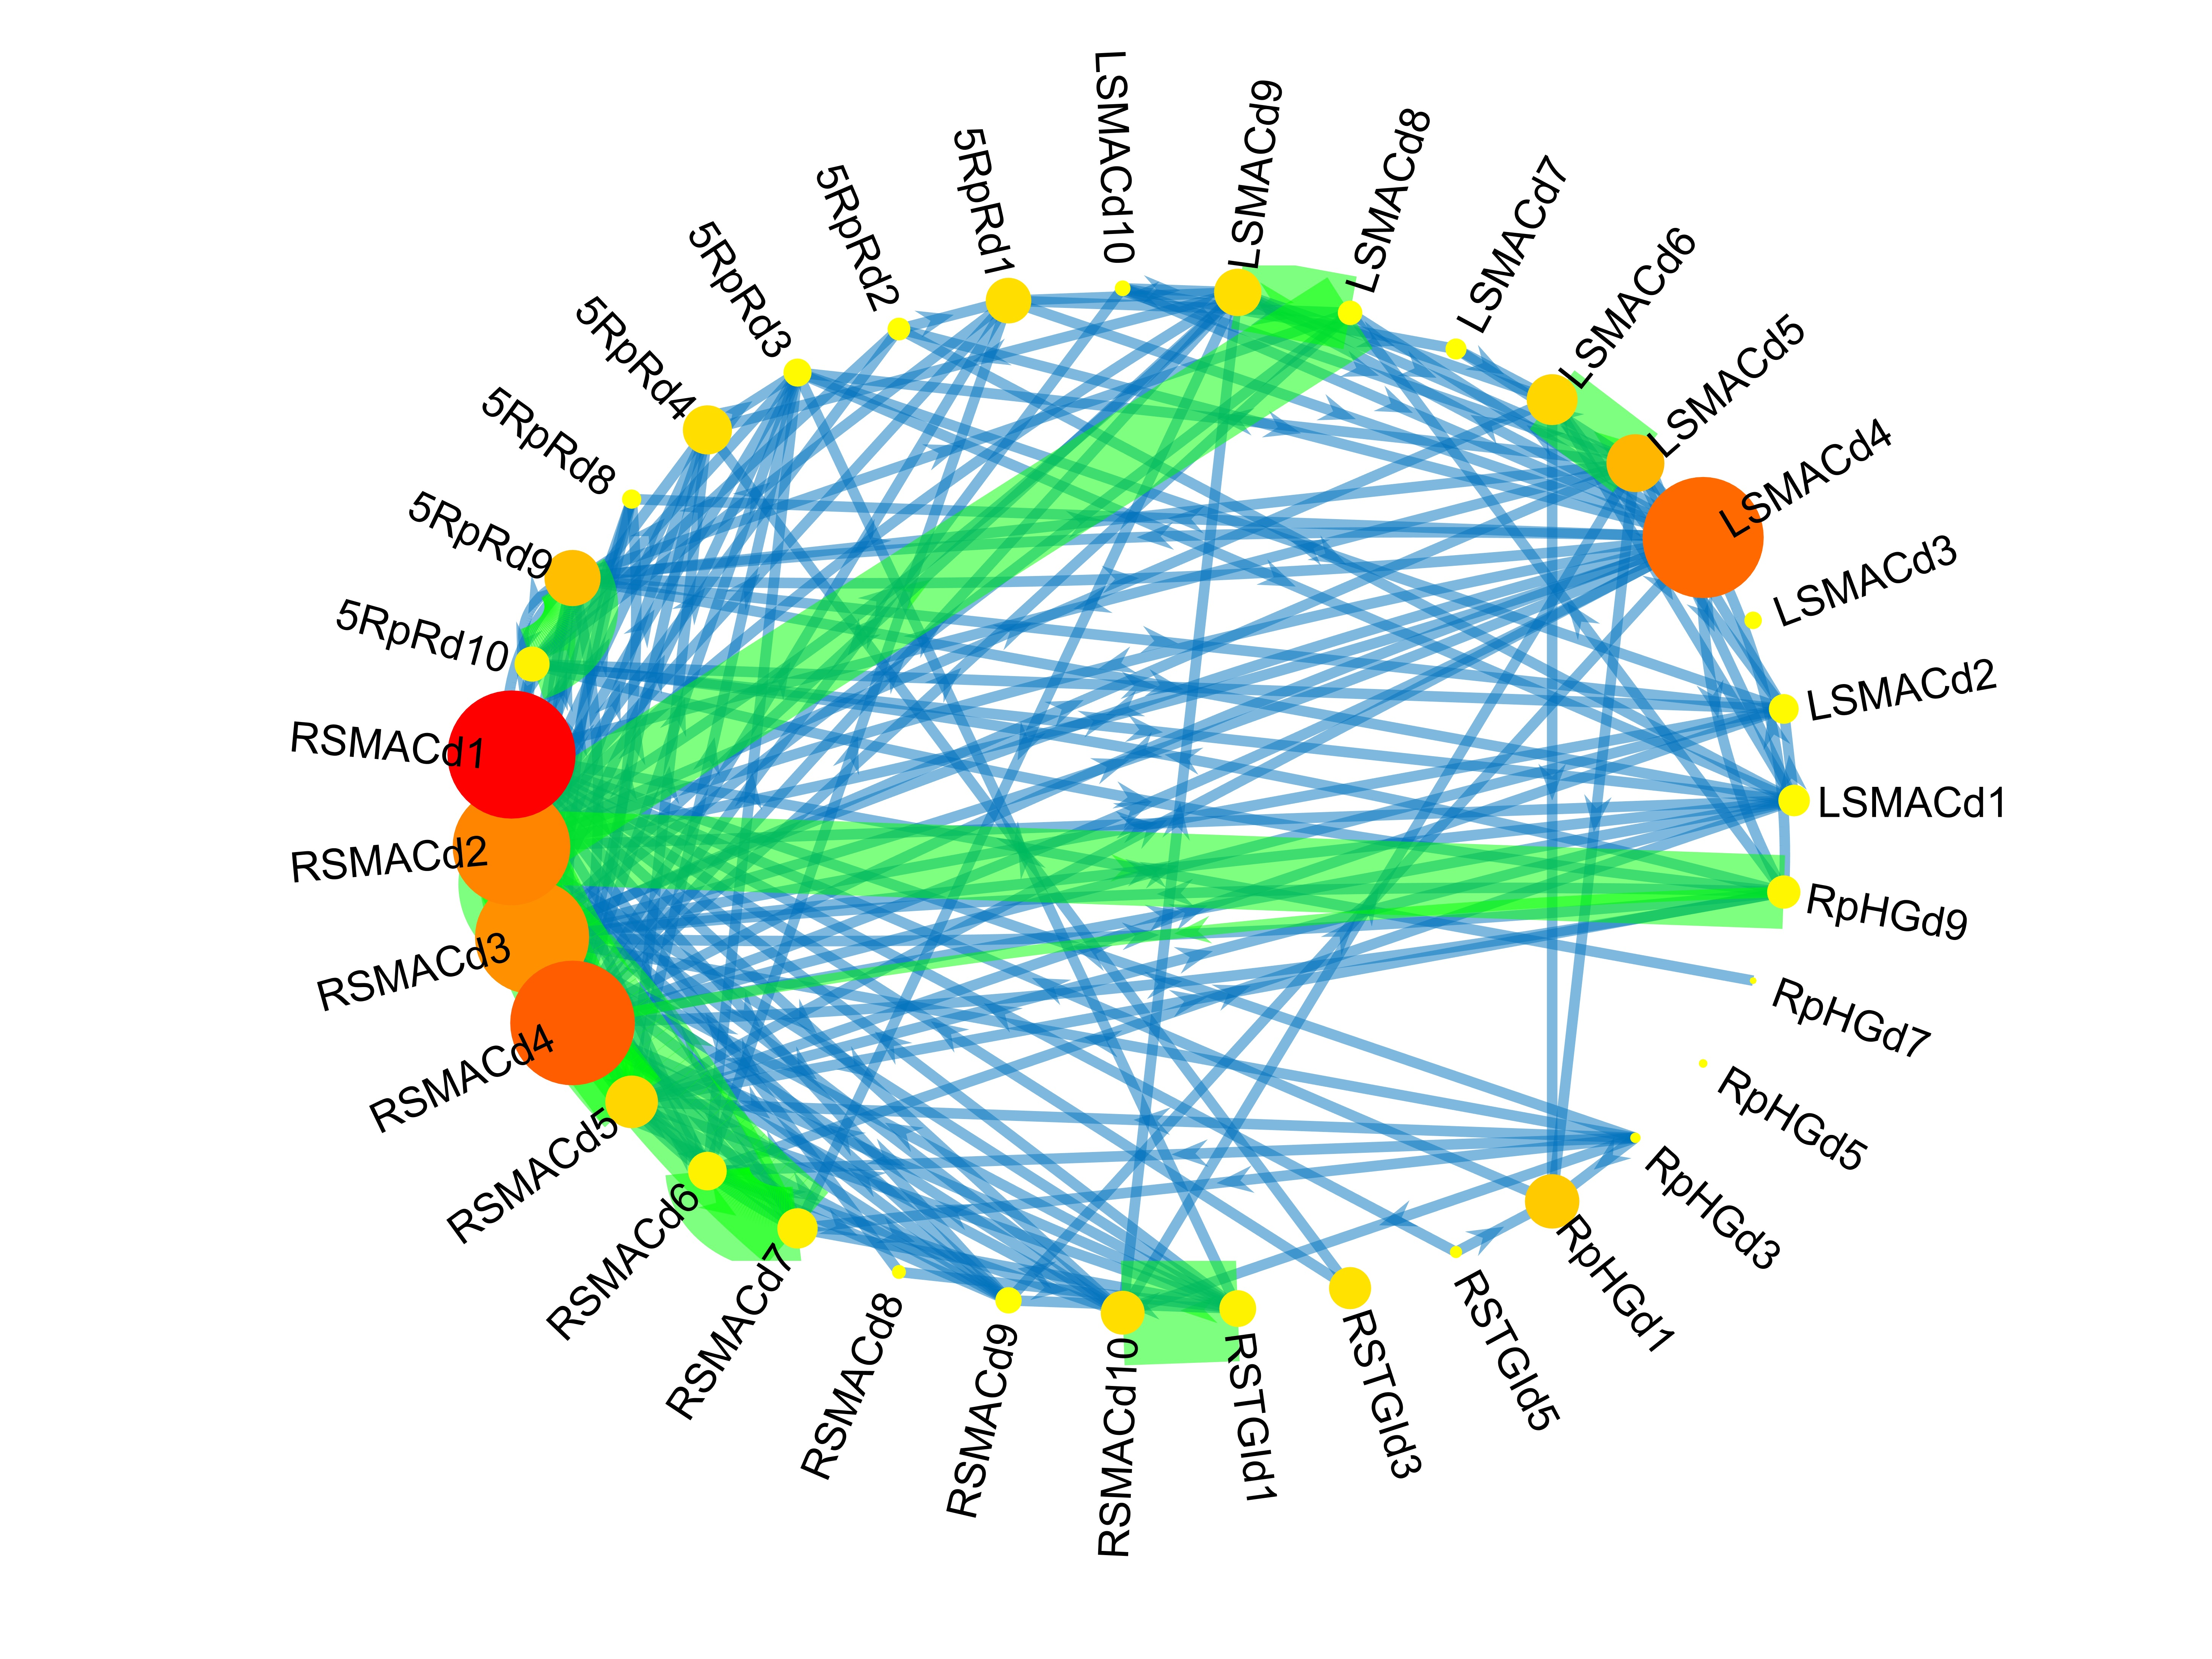
\includegraphics[width=13cm]{Plots/Patient_C_betweenness_ieeg.jpg} }}%
    
    b) {{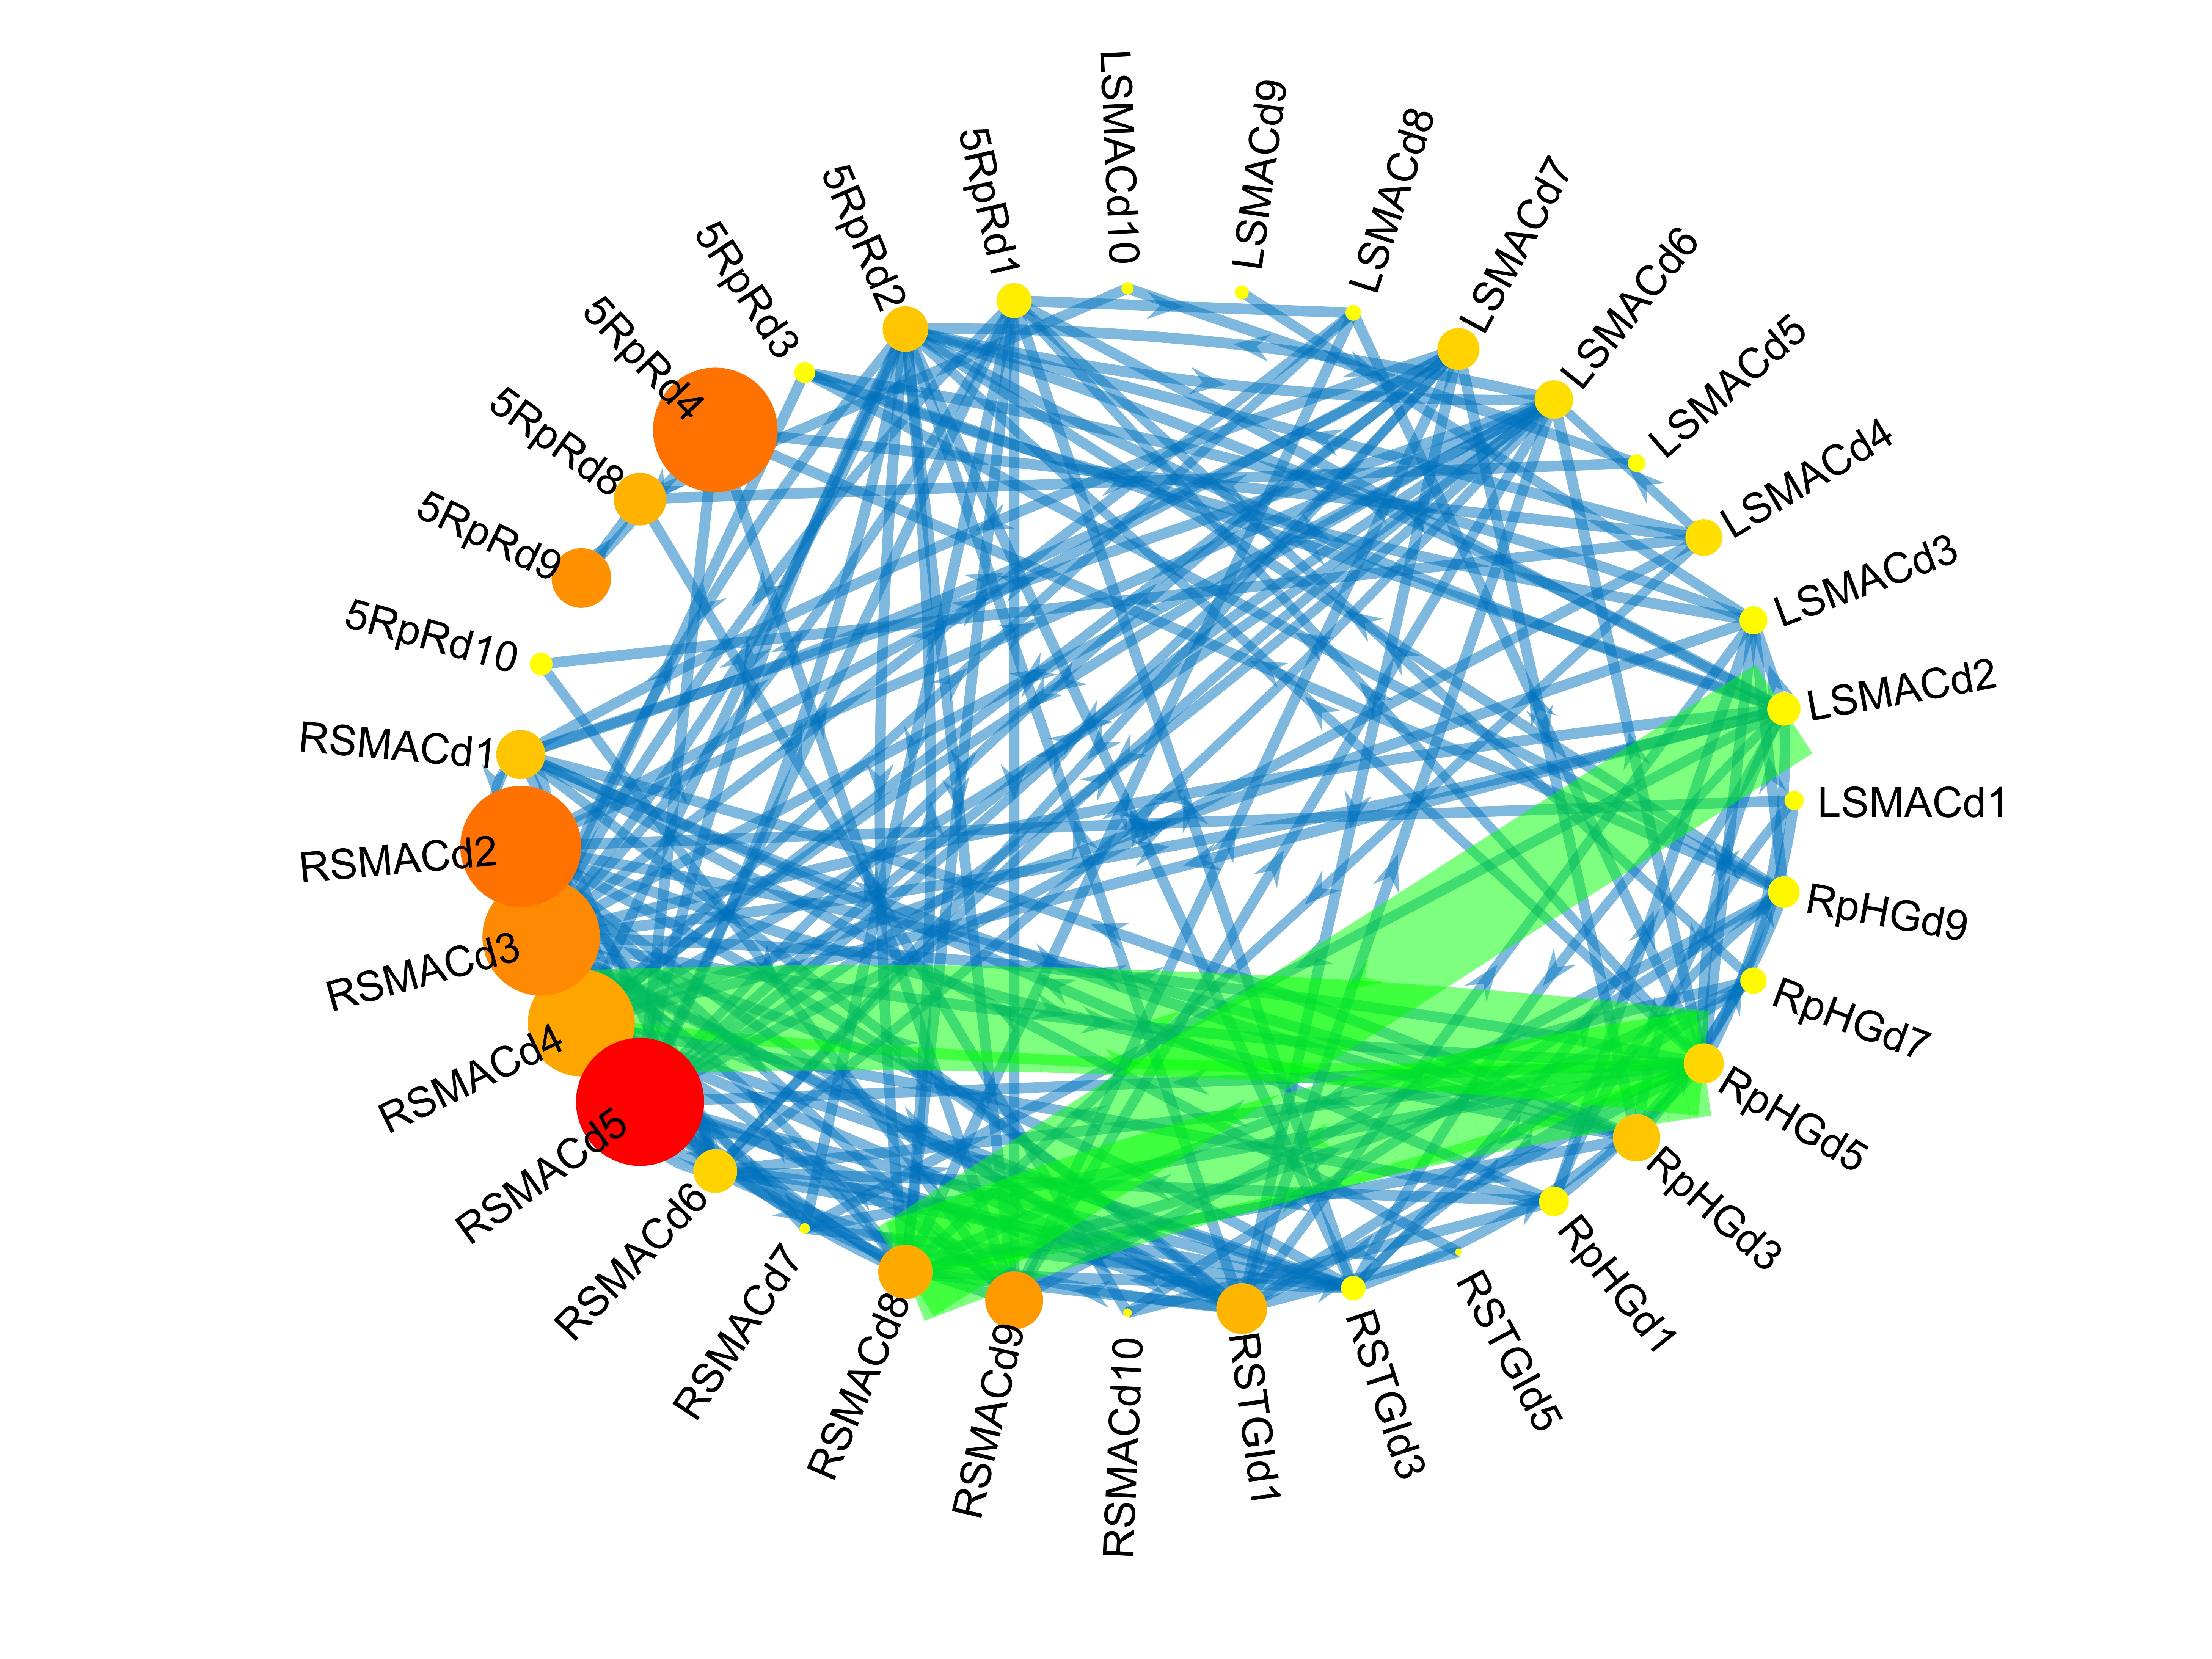
\includegraphics[width=13cm]{Plots/Patient_C_betweenness_fmri.jpg} }}%
    \caption{Betweenness measure computed from time domain Granger causality as adjacency matrix for a) iEEG, and b) fMRI. Red represents the node with the highest measure value and green represents the strongest edge or the connectivity strength. Strongest connection is observed between RSMAcd and LSMAcd electrodes.}%
    \label{fig:betweenness_fmri_eeg}%
\end{figure}


\begin{table}[]
\renewcommand{\arraystretch}{1.2} % Default value: 1
\setlength{\tabcolsep}{2pt} % Default value: 6pt
\centering
\begin{tabular}{|l|c|c|c|c|c|c|}
\hline
\multirow{2}{*}{\textbf{Measures}} & \multicolumn{2}{c|}{\textbf{4x4x4$mm^3$}}                                     & \multicolumn{2}{c|}{\textbf{6x6x6$mm^3$}}                                     & \multicolumn{2}{c|}{\textbf{8x8x8$mm^3$}}                                     \\ \cline{2-7}
                                   & \multicolumn{1}{l|}{\textbf{RSMAcd3}} & \multicolumn{1}{l|}{\textbf{RSMAcd4}} & \multicolumn{1}{l|}{\textbf{RSMAcd3}} & \multicolumn{1}{l|}{\textbf{RSMAcd4}} & \multicolumn{1}{l|}{\textbf{RSMAcd3}} & \multicolumn{1}{l|}{\textbf{RSMAcd4}} \\ \hline
Total GC                           & 17\%                                  & 27\%                                  & -                                     & \textbf{1\%}                          & \textbf{3\%}                          & \textbf{1\%}                          \\ \hline
Betweenness                        & -                                     & -                                     & -                                  & 17\%                                  & \textbf{5\%}                          & \textbf{6\%}                          \\ \hline
Degree                             & -                                     & -                                     & -                                     & \textbf{0.2\%}                        & \textbf{13\%}                         & \textbf{1\%}                          \\ \hline
Incloseness                        & -                                     & -                                     & -                                     & \textbf{1\%}                          & \textbf{4\%}                          & \textbf{3\%}                          \\ \hline
ClusteringCoef                    & -                                     & -                                     & -                                     & 26\%                                  & \textbf{4\%}                          & 17\%                                  \\ \hline
\end{tabular}
	\caption{The voxel wise analysis of gray matter on epileptic patients. SO electrodes RSMAcd3 and RSMAcd4 are ranked as percentage for four graph measures. N is the total number of voxels for each dimension. `-' represents non-significant results. Both SO electrodes lie within top 5\% for 8*8*8 $mm^3$ voxel dimension}
	\label{table:voxelwise_summary}
\end{table}

\subsection{Voxelwise analysis}
Previous computation was based upon the ROI extraction using spherical mask around the MNI coordinates. Some areas or voxels can be missed between two electrode contacts, which could potentially be the true seizure onzet zone. These regions can remain undetected using neuroimaging techniques or iEEG. To consider such regions, we varied the voxel dimensions (4x4x4 $mm^3$, 6x6x6 $mm^3$ and 8x8x8 $mm^3$) and computed the pairwise Granger causality between every other voxels in the gray matter.

\subsubsection{Rank of SO voxels}
The rankings of SO voxels among the total number of source voxels are shown in Table \ref{table:voxelwise_summary}. As we increase the voxel dimensions, total number of voxels in each voxel dimension decreases (15,462 voxels with $4*4*4mm^3$, 4,552 in 6*6*6 $mm^3$ and 1,959 in 8*8*8 $mm^3$). We ranked our result for each voxel in descending order of their magnitude for all measures. The percentage value is computed as the percent of rank of the SO electrode to the total number of voxels. As summarized in the table, the SO electrode RSMAcd4 is ranked within the top 1\% for 6x6x6 $mm^3$ voxel dimension for Total GC, Degree and Incloseness measures. Both the SO electrodes - RSMAcd3 and RSMAcd4 are among top 5\% in almost all measures for 8*8*8 $mm^3$ voxel dimension. '-' denotes that the result is not significant. The analysis for 10*10*10 $mm^3$ voxel dimension was not significant and it is not included in the table.


\begin{table}[]
\renewcommand{\arraystretch}{1.2} % Default value: 1
\setlength{\tabcolsep}{8pt} % Default value: 6pt
\centering
\begin{tabular}{|l|r|r|r|r|r|}
\hline
\multicolumn{1}{|c|}{\textbf{Measures\textbackslash MNI}} & \multicolumn{1}{c|}{\textbf{(2, -2, 40)}} & \multicolumn{1}{c|}{\textbf{(6, -6, 32)}} & \multicolumn{1}{c|}{\textbf{(6, 6, 40)}} & \multicolumn{1}{c|}{\textbf{(6, 6, 44)}} & \multicolumn{1}{c|}{\textbf{(10, 6, 44)}} \\ \hline
\textbf{Total GC}                                                & 79                                        & 173                                       & 88                                       & 506                                      & 244                                       \\ \hline
\textbf{Betweenness}                                             & 118                                       & 89                                        & 8                                        & 269                                      & 234                                       \\ \hline
\textbf{Degree}                                                  & 253                                       & 270                                       & 407                                      & 351                                      & 909                                       \\ \hline
\textbf{Incloseness}                                             & 88                                        & 392                                       & 154                                      & 178                                      & 709                                       \\ \hline
\textbf{Top R}                                                   & 79                                        & 89                                        & 8                                        & 178                                      & 234                                       \\ \hline
\textbf{Top ranked \%}                                           & 0.5\%                                     & 0.6\%                                     & 0.1\%                                    & 1.2\%                                    & 1.5\%                                     \\ \hline
% \textbf{Avg rank}                                                & 135                                       & 231                                       & 164                                      & 326                                      & 524                                       \\ \hline
% \textbf{Avg rank \%}                                            & 0.9\%                                     & 1.5\%                                     & 1.1\%                                    & 2.1\%                                    & 3.4\%                                     \\ \hline
\end{tabular}
	\caption{Rank of voxels located in the boundary of  8*8*8 $mm^3$ voxel in the site of SO electrodes}
	\label{table:rank_of_voxels_nearby_soe}
\end{table}


\subsubsection{Neighborhood around SO voxels}
The SO electrodes were ranked at the top for voxel dimension 8*8*8 $mm^3$ but not for 4*4*4 $mm^3$. This could be because the targeted voxel existed beyond the 4 mm voxel dimension but inside 8 mm. For the finer details, we focused on the spherical volume of radius 8mm around the center of SO electrodes as determined above and consider all 4x4x4 voxels within this boundary, and checked their rankings in the 4mm dimension, consisting of 15,562 voxels.

Table \ref{table:rank_of_voxels_nearby_soe} shows the ranks of 5 voxels that were constantly ranked highest for all 4 measures out of the 15,562 voxels. The measure for which the rank is topmost (i.e. lowest number in table) is selected as the top ranked voxel and its percentage is shown in the top ranked percentage row. The voxel with MNI coordinate (6, 6, 40) was ranked $8^{th}$ out of 15,462 voxels for the betweenness measure. This voxel is also ranked within top 5 percentage for all other measures. Similarly the nearby voxel (2, -2, 40) was ranked among top 5 percentage for total GC and betweenness among these 5 voxels. However, it is possible that the voxel (6, 6, 40) represents the prime voxel for seizure onset, being located very close to the identified SO electrode RSMAcd4, and ranked at the 0.05 percentile for the entire brain using the betweenness measure. 


\begin{figure*}
\centerline{
	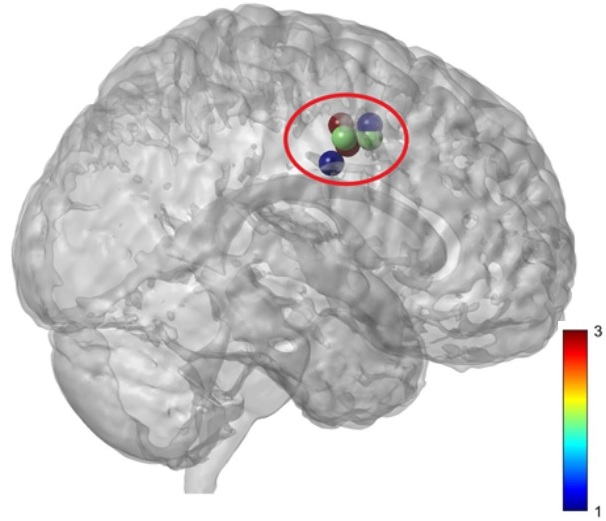
\includegraphics[height =3in]{Plots/top_voxels.jpg}
	}
	\caption{ Top voxels according to total causal flow and three graph measures located within the boundary of 8*8*8 $mm^3$ voxels dimension. Two red dots are SO voxels - RSMAcd3 and RSMAcd4 with voxel dimension 4*4*4 dimension. (2,-2,40) and (6, 6, 40) are represented as green dots. Blue dots are the other three voxels.
	\label{fig:top_voxels}
}
\end{figure*}

\begin{figure*}
\centerline{
	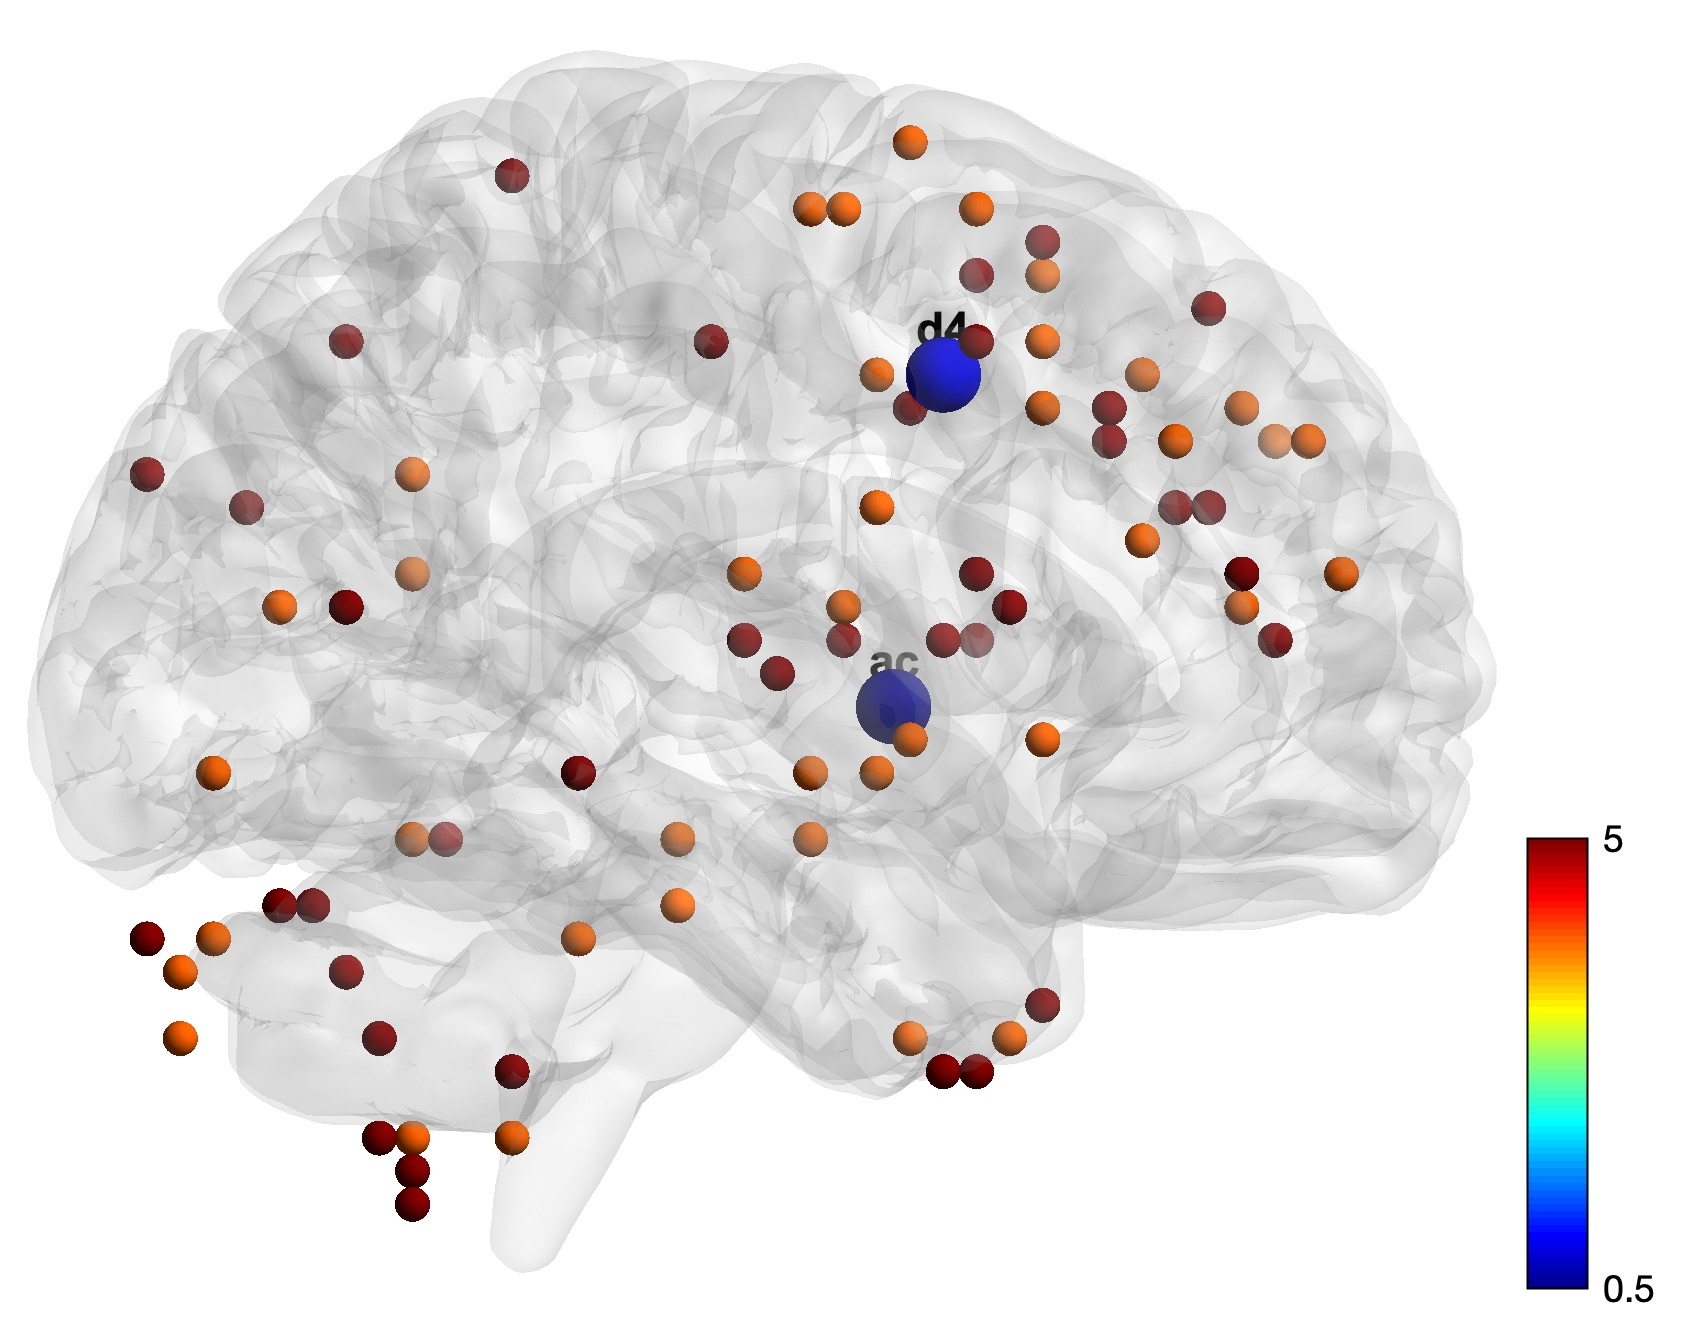
\includegraphics[height =3in]{Plots/Patient_C_eegfmri_voxel_cluster.jpg}
	}
	\caption{ The top 80 connections from the $8^{th}$ top ranked (6, 6, 40) voxel of over 12,000. The outflow clusters are observed in frontal lobes, cerebellum, basal ganglia and thalamus.
	\label{fig:top_voxel_cluster}
}
\end{figure*}

%This voxel lies at d4 and anterior commisure (ac) is the centre or the reference point of the brain.

Figure \ref{fig:top_voxels} illustrates the top voxels of 4*4*4 $mm^3$ voxel dimension located within the boundary of 8*8*8 $mm^3$ voxel dimension right in the location of SO electrodes. 

%We observed that different voxels were ranked highest for different measures instead of single voxels as the maximum of all measures. The averages of these voxels might have been the reason behind the maximum value and consistently significant result for 8*8*8 $mm^3$ voxels dimension. We were able to find the seizure onset voxel in voxel dimensions as small as 4*4*4 voxel $mm^3$.

Figure \ref{fig:top_voxel_cluster} shows the strongest connections from the top ranking voxel (8 out of 15,000) to the whole brain. The connections of this voxel cluster around frontal lobes, cerebellum, basal ganglia and thalamus. These areas have a major role in cognition, decision making and motor control. This result demonstrates the connection between seizure origin and other areas. The impairment of these clustered areas could be associated with the seizure symptoms.


\section{Discussion}
\label{sec:discussion}
In this study, we used quantitative techniques based on Granger causality and graph theory to study the correlation between iEEG and BOLD signals from resting state fMRI. Our results showed that the iEEG electrode contacts with the strongest infra-slow EEG signal correlated with the spontaneous BOLD fluctuations in corresponding location. The voxels within a small radius of the seeded location were constantly significant for total causal flow and directed centrality measures like betweenness, degree and incloseness. Individual voxel analysis within this radius showed a highly significant clustering based on various measures when compared to other voxels throughout the entire brain.

We compared the causal relationship of the total causal flow and sink activity between the infra-slow interictal iEEG time-series and the corresponding fMRI BOLD signal. However, causal relationship was not overlapped for the same range of infra-slow frequency range. The infraslow frequency range considered for BOLD signal was longer than that for iEEG. Based on our multiple experiments on different frequency ranges, we found that the frequency range 0.01-0.2 Hz in iEEG and 0.08-0.8 Hz in fMRI have the highest coupling between each other and the SO electrodes. This result could be patient specific, and multiple patients have to be studied to find the average overlap range of infraslow frequency between iEEG and fMRI.

The voxelwise analysis of whole brain showed that the voxels in the proximity of seeded locations resulted in the top rank for the computed quantitative measures.The electrical activity recorded in SO iEEG electrodes might have been influenced by these cluster of voxels as \citep{menon1996spatio} illustrated that the distribution of coherence values differed from background level at interisite distances of 1 and 1.4 cm for iEEG electrodes. Prolonged seizure freedom by a small laser resection strongly supports the iEEG indications that the presumed focus did indeed include the true seizure onset zone. 

%The reason for the patient to be seizure free could be the removal of this area along with the targeted brain area by laser surgery. The other reason for this significant cluster could be due to the mismatch between seizure onset zone (SOZ) and the corresponding seeding in fMRI. The SOZ, identified in fMRI scan, could have been shifted by a few millimeters due to swelling or the invasion by implanted electrodes.

We acknowledge the challenges in comparing EEG and BOLD signals. Few previous studies have used functional connectivity measures in the two signals,  similar to our approach. Instead, we follow the same methods of functional connectivity method - Granger causality and graph measures, for both iEEG and BOLD signals, similar to our analysis of high-frequency infra-slow iEEG time-series for different phases of epilepsy. 

The iEEG and BOLD signals not being recorded simultaneously is another challenge. As discussed by Aghakhani and team, the BOLD signal from true seizure onset areas could be distorted in simultaneous iEEG-fMRI due to implanted electrodes \citep{aghakhani2015co}. The time of acquisition of fMRI and iEEG signals differed by several months in our study. Neuroimaging and iEEG studies have confirmed that significant progression of the epilep- togenic process might progress over several years in epilepsy \citep{walker2002disease}. However, the locations of the SOZ appear nearly identical in our dataset.

The other challenges include the computation time for connectivity measures with a large number of voxels. We limited our analysis to $4_{mm}^3$ voxel dimensions as the computation boundary of the cluster computer in our lab. The number of voxels would increase to hundred of thousands as we increase the resolution to $2_{mm}^3$ voxels, the highest resolution of fMRI with present day scanners. The correlations between the neighboring voxels can be profound at this level and the result could be compromised. We also limited our study of causality to pairwise parametric Granger causality, instead of a non-parametric method for the same reason. However, we determined model order by comparing spectral power between parametric and non-parametric methods for the validation of autoregressive model fitting of the data. These two issues related to computation time could be resolved in the future with more efficient algorithms and more powerful computing resources. 

Despite these challenges and limitations, we are able to demonstrate that using the intracranial ictal EEG recording as a seed, the infraslow EEG activity is highly correlated with the corresponding voxels of the resting state functional MRI (rsfMRI) recorded months before. As such, intracranial EEG has the potential to be used as a seed in the rsfMRI to characterize the epilepsy focus and connections of the epilepsy network throughout the entire brain at milimeters resolution. 

Nonetheless, the fine detail mapping of the epilepsy network presented in this study requires further extensive testing and analysis to determine the optimal methods for characterizing and displaying the results. As with other applications of RSfMRI, causal analysis, and graph theory, a great variety of techniques are feasible. Obvious questions of importance include the percentage of potential epilepsy surgery patients in whom the focus can be this precisely defined, including those with visible lesions or possible tandem foci; and whether combining them with cluster analysis may allow the application of these techniques to the interictal resting state fMRI alone.